\documentclass[11pt]{article}
\usepackage{fullpage}
\usepackage{enumitem}
\usepackage{pdfpages}
\usepackage{graphicx}
\begin{document}
\author{Benjamin Sorenson} \title{Assignment 2}
\maketitle

\begin{enumerate}[label=\bfseries Question \arabic*:]
\item
  \begin{enumerate}
  \item Formulate the problem:
    \begin{description}
    \item[As a complete-state] \hfill \\
      \begin{description}
      \item[State Space] \hfill \\
        All possible arrangements of \(N\) guests around the table.
      \item[State Representation] \hfill \\
        Each state could be represented as an array \(A\)
        of integers in \(\left[0, N\right]\)---\(0\)
        would represent and empty seat at the table, and any number
        \(k \ge 1\)
        in position \(i\)
        (i.e., \(A\left[i\right]=k\))
        would mean that person \(k\) is seated at position \(i\).
      \item[Initial State] \hfill \\
        The initial state could be any arrangement of \(N\)
        guests at the table
      \item[Goal Test] \hfill \\
        All guests are seated, and the total group satisfaction cannot
        be improved by changing the position of any one of the guests.
      \item[Actions] \hfill \\
        \begin{description}
        \item[\(INSERT-RIGHT(S,i,j)\)]
          given a state \(S\),
          assign guest in position \(i\)
          to position \(j\),
          and shift the guests to the right of \(j\)
          right one position.
        \item[\(INSERT-LEFT(S, i, j)\)]
          Similar to \(INSERT-RIGHT\),
          but guests to the left of \(j\)
          are shifted left one position.
        \item[\(SWAP(i, j)\)]
          Swap guest in position \(i\) with guest in position \(j\)
        \end{description}
      \end{description}
    \item[As an incremental formulation] \hfill \\
      \begin{description}
      \item[State Space] \hfill \\
        All possible arrangements of \(0 \le n \le N\)
        guests around the table
      \item[State Representation] \hfill \\
        Same as above
      \item[Initial State] \hfill \\
        No guests seated at the table.

      \item[Actions] \hfill \\
        All the same actions as above with the addition of
        \begin{description}
        \item[\(SEAT(S, k, i)\)]
          given a state \(S\) seat person \(k\) in open position \(i\)
        \end{description}
      \item[Goal Test] \hfill \\
        Same as above
      \end{description}
    \end{description}
  \item The advantage of the complete-state formulation is that the
    state space is smaller than the incremental formulation. There are
    ``only'' \((n-1)!\)
    possible state in the complete-state formulation, and there are
    \(\sum_{i=0}^{N-1}{i!}\)
    states in the incremental formulation. The incremental solution
    might be easier to solve since it's essentially the same problem
    as the complete-state formulation, but we can construct the
    initial state.
  \item Since we're trying to maximize \(Pleasure(i, j)\),
    in order to be admissible, our heuristic has to be
    \( \ge \max\left\{Pleasure(i, j)\right\}\)--an
    attempt at this might be
    \(h(n) = N \cdot Pleasure(i_{\max}, j_{\max}) \)
    where \(i_{max}\)
    and \(j_{max}\)
    are the guests in state \(S\)
    who derive the most pleasure from the arrangement.  This isn't
    admissible since in the case when there are two guests, we can't
    guarantee that \(h(n)\) is an overestimate.
  \end{enumerate}
\item
  \begin{enumerate}
  \item No, greedy best-first search can at best find a solution equal
    in cost to what \(A^{*}\)
    will find since \(A^{*}\)
    is guaranteed to find an optimal solution if one exists.  For
    example, using the example graph from class, the green path shows
    the path found (eventually) by \(A^{*}\)
    search, and the red path shows where greedy best-first deviated
    from the optimal path
\par\centerline{
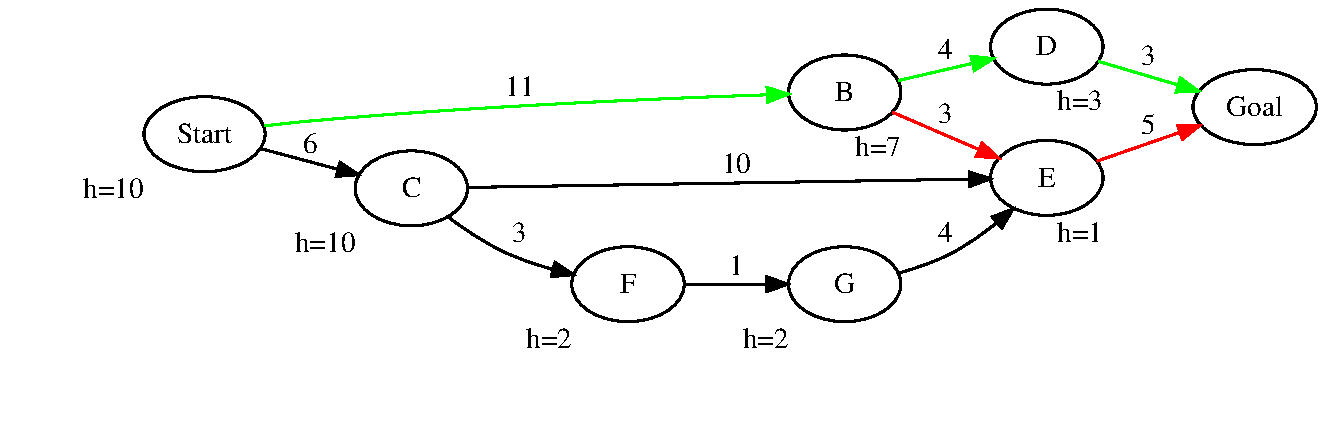
\includegraphics[scale=.75]{classgraph-2a.pdf}
}

\item Yes, in general greedy best-first search will be faster
  \(A^{*}\)
  search since it stops as soon as it reaches the goal.  \(A^{*}\)
  search, however, will continue until it has found the lowest cost
  path. \(A^{*}\)
  can get lucky and find the lowest cost solution as fast a greedy
  best-first search, but in general it will be slower.  It's difficult
  to show this graphically, but again, taking the example from class,
  \(A^{*}\)
  search had to expand every node at least once (\(E\)
  three times) before finding the optimal path. By contrast, greedy
  best-first search expanded just two nodes.
\item When \(h(n)=-2 \cdot g(n)\),
  greedy best-first search behaves like a hill climbing algorithm.  It
  evaluates each node by assigning it a negative value equal to twice
  the path cost of reaching that node.  Thus, taking the node that
  most increases the total cost---much like hill-climbing. The
  following example show best-first search on with \(h(n)\)
  defined as above. Since \(h(n)\)
  depends on \(g(n)\),
  the value of \(h(n)\) is shown only for children of expanded nodes.
\par\centerline{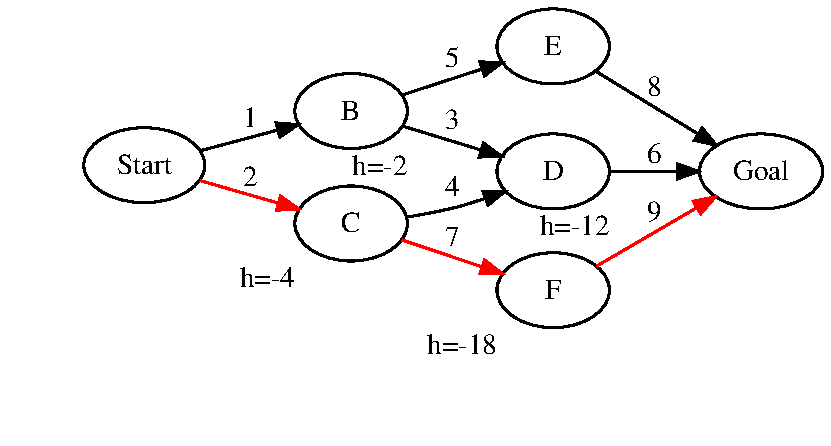
\includegraphics[scale=.75]{neg-2-hn.pdf}}
\end{enumerate}
\item
  \begin{enumerate}
  \item Yes. Since we are only multiplying \(f(n)\)
    by a constant, the ordering of the nodes and path costs remains
    unchanged so not only will \(A^{*}\)
    still find an optimal path, but its behavior will be exactly the
    same.  See the following example.  The first path taken is in red,
    and the second, optimal path taken is in green.  The first graph
    shows \(f(n)\)
    defined as it usually is, and the second graph shows \(f(n)\)
    defined as \(f(n)=3 \cdot g(n) + 3 \cdot h(n)\).
    \[f(n) = g(n) + h(n)\]
\par\centerline{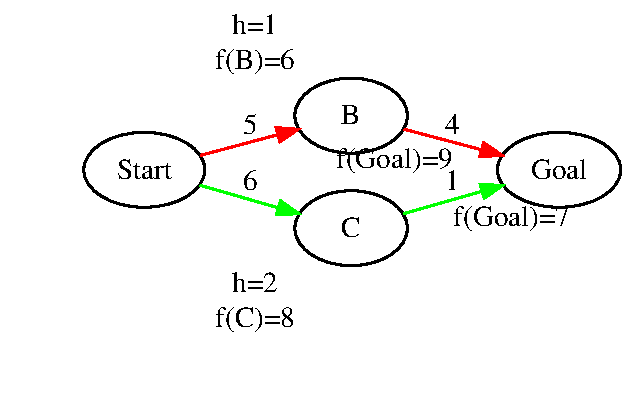
\includegraphics[scale=.75]{fgn.pdf}}
    \[f(n) = 3 \cdot g(n) + 3 \cdot h(n)\]
\par\centerline{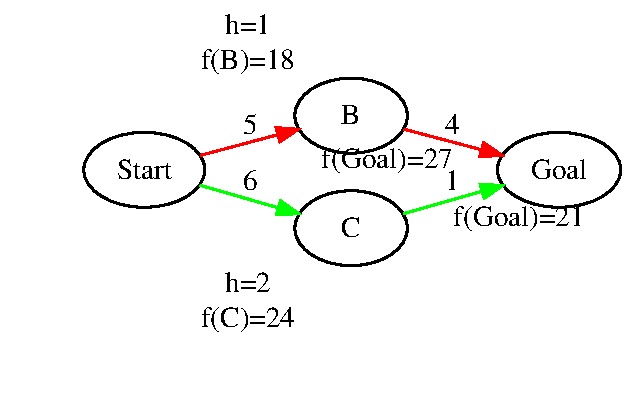
\includegraphics[scale=.75]{f3g3n.pdf}}
  \item I will assume that \(0 \le w \le 1\).
    From part (a), it is easy to see that a value of \(w=.5\)
    will still guarantee an optimal solution, \(w=0\)
    (uniform cost search) will guarantee an optimal solution, but
    \(w=1\)
    (greedy best-first search), will not. From this alone, we can
    conclude that the answer depends on the value of \(w\)
  \item \(g(n)\)
    and \(h(n)\)
    control the shape of search contours of the search---emphasizing
    \(g(n)\)
    widens the contours, and emphasizing \(h(n)\)
    narrows the contours.
  \end{enumerate}
\item
  \begin{enumerate}
  \item \(h_3(n) =\max\{h_1(n),h_2(n) \} \)
    is admissible. Since both \(h_1\)
    and \(h_2\)
    are admissible, the maximum of of \(h_1\)
    and \(h_2\)
    will also be admissible.  I would use \(h_3\)
    instead of either \(h_1\)
    or \(h_2\)
    because \(h_3\)
    will be at least as accurate as either \(h_1\)
    or \(h_2\)
    alone---the more accurate the heuristic, the more narrow the
    search becomes around the optimal path.
  \item \(h_4(n) = \max\{h_1(n), 1.1 \cdot h_2(n) \}\)
    may not be admissible.  Since \(1.1\cdot h_2(n)\ \ge h_2(n)\),
    \(\max \{h_1(n), 1.1\cdot h_2(n)\}\)
    may overestimate the cost to reach the goal.
  \item \(h_5(n) = \min\{h_1(n), 2 \cdot h_2(n)\}\)
    is admissible since \(h_5(n) \le h_1(n)\)
  \item \(h_6(n)=\frac{h_1(n) + h_2(n)}{2}\)
    is admissible since \(h_6(n) < h_3(n)\)
  \item \(h_7(n) = \frac{h_1(n)}{3} + \frac{h_2(n)}{2}\)
    is admissible since \(h_7(n) < h_6(n)\)
  \end{enumerate}
\item
  \begin{enumerate}
  \item Suppose that \(A^{*}\)
    left some node with \(f(n) < C^*\)
    closed after finding the optimal solution. By the formulation of
    the algorithm, it would then expand the node, and continue.
  \item Breadth-first search will expand all nodes until the goal is
    reached---completeness is unrelated to paths cost.
  \item \(A^*\)
    cannot be used for online search. In order to search a state space
    \(A^*\)
    must be used in a n environment where the resultant state of an
    action on the current state can be known.  By definition, the
    resultant state of an action in on-line search cannot be known
    prior to the action being completed. Therefore \(A^*\)
    search cannot be used for on-line search.
  \end{enumerate}
\end{enumerate}
\end{document}
